%% Seuraava rivi varoittaa vanhoista tai huonoista latex komennoista
\RequirePackage[l2tabu, orthodox]{nag}

%% Käytä toinen näistä:
%% ensimmäinen, jos käytät pdflatexia, joka kääntää tekstin suoraan
%% pdf-tiedostoksi (kuvat on oltava jpg- tai pdf-tiedostoina)
%% toinen, jos haluat tuottaa ps-tiedostoa (käytä eps-formaattia kuville,
%% alä käytä ps-muotoisia kuvia!)
%%
\documentclass[finnish,12pt,a4paper,pdftex,elec,utf8]{aaltothesis}
%\documentclass[finnish,12pt,a4paper,dvips]{aaltothesis}

%% Kirjoita y.o. \documentclass optioiksi
%% korkeakoulusi näistä: arts, biz, chem, elec, eng, sci
%% editorisi käyttämä merkkikoodaustapa: utf8, latin1
%%

%% Käytä näitä, jos kirjoitat englanniksi. Katso englanninokset tiedostosta
%% thesistemplate.tex.
%\documentclass[english,12pt,a4paper,pdftex,elec,utf8]{aaltothesis}
%\documentclass[english,12pt,a4paper,dvips]{aaltothesis}

\usepackage{graphicx}

%% Matematiikan fontteja, symboleja ja muotoiluja lisää, näitä tarvitaan usein
\usepackage{amsfonts,amssymb,amsbsy}

%% Jos et jostain syystä pidä, miten alla oleva hyperref-paketti käyttää
%% fontteja, värejä yms., käytä tämän paketin makroja muuttamaan
%% fonttimäärittelyt. Katso paketin dokumentaatiota. Paketti määrittelee
%% \url-makron, joten ota paketti käyttöön, jos et käytä hyperref-pakettia.
%%
%\usepackage{url}

%% Saat pdf-tiedoston viittaukset ja linkit kuntoon seuraavalla paketilla.
%% Paketti toimii erityisen hyvin pdflatexin kanssa.
%%
\usepackage{hyperref}
\hypersetup{pdfpagemode=UseNone, pdfstartview=FitH,
colorlinks=true,urlcolor=red,linkcolor=blue,citecolor=black,
pdftitle={Pieni maailma verkostot},pdfauthor={Ossi Galkin},
pdfkeywords={Pieni maailma verkostot, pienen maailman verkostot, pieni maailma -verkostot, kompleksiset verkostot, sosiaaliset verkostot, kompleksiset systeemit, dynaamiset verkostot}}

%% Omat säädöt

\graphicspath{{Kuvat/}}
\usepackage{gensymb}
\usepackage[utf8]{inputenc}

\usepackage[%
backend=bibtex % biber or bibtex
% ,style=authoryear % Alphabeticalsch
,style=numeric-comp % numerical-compressed
,sorting=none % no sorting
,sortcites=true % some other example options ...
,block=none
,indexing=false
,citereset=none
,isbn=true
,url=true
,doi=true % prints doi
,natbib=false % if you need natbib functions
,dateabbrev=false
]{biblatex}
\addbibresource{Viitteet.bib}
%\bibliography{viitteet}


\DefineBibliographyStrings{finnish}{%
    url = {Saatavissa:},
	urlseen = {Viitattu}
}

\DeclareFieldFormat{url}{\bibstring{url}\space\url{#1}}
\DeclareFieldFormat{journaltitle}{\mkbibemph{#1}, verkkolehti,} % italic journal title with comma
%\DeclareFieldFormat{volume}{vol. {#1}, } 
\DeclareFieldFormat{issue}{nro {#1},} 


\renewbibmacro*{volume+number+eid}{%
\addnbspace\textnormal{vol. }
  \printfield{volume}%
  \setunit{\addcomma\space}}
\DeclareFieldFormat[article]{number}{\mkbibparens{#1}}


% Seuraava haxi poistaa sulut päivämäärän ympäriltä, tuo voi rikkoa muita juttuja viitteissä...
\renewcommand{\bibopenparen}{\addcomma\addspace}
\renewcommand{\bibcloseparen}{\addcomma\addspace}

%\renewbibmacro*{volume+number+eid}{%
%\addnbspace\textnormal{vol. }
%  \printfield{volume}%
%  \setunit*{\adddot}% DELETED
%\addcomma
%  \setunit*{\addnbspace}% NEW (optional); there's also \addnbthinspace
%  \addnbspace\textnormal{nro }
%  \printfield{number}%
%  \setunit{\addcomma\space}%
%  \printfield{eid}}
%\DeclareFieldFormat[article]{number}{\mkbibparens{#1}}

%% Kaikki mikä paperille tulostuu, on tämän jälkeen
\begin{document}

%% Korjaa vastaamaan korkeakouluasi, jos automaattisesti asetettu nimi on
%% virheellinen
%%
%% Change the school field to specify your school if the automatically
%% set name is wrong
% \university{aalto-yliopisto}
% \school{Sähkötekniikan korkeakoulu}

%% Vain kandityölle: Korjaa seuraavat vastaamaan koulutusohjelmaasi
%%
\degreeprogram{Automaatio- ja systeemitekniikka}
%%

%% VAIN DI/M.Sc.- JA LISENSIAATINTYÖLLE: valitse laitos,
%% professuuri ja sen professuurikoodi.
%%
% \department{Radiotieteen ja -tekniikan laitos}
% \professorship{Piiriteoria}
%%

%% Valitse yksi näistä kolmesta
%%
\univdegree{BSc}
%\univdegree{MSc}
%\univdegree{Lic}

%% Oma nimi
%%
\author{Ossi Galkin}

%% Opinnäytteen otsikko tulee tähän ja uudelleen englannin- tai
%% ruotsinkielisen abstraktin yhteydessä. Älä tavuta otsikkoa ja
%% vältä liian pitkää otsikkotekstiä. Jos latex ryhmittelee otsikon
%% huonosti, voit joutua pakottamaan rivinvaihdon \\ kontrollimerkillä.
%% Muista että otsikkoja ei tavuteta!
%% Jos otsikossa on ja-sana, se ei jää rivin viimeiseksi sanaksi
%% vaan aloittaa uuden rivin.
%%
\thesistitle{Pieni maailma verkostot}

\place{Espoo}

%% Kandidaatintyön päivämäärä on sen esityspäivämäärä!
%%
\date{3.5.2016}

%% Kandidaattiseminaarin vastuuopettaja tai diplomityön valvoja.
%% Huomaa tittelissä "\" -merkki pisteen jälkeen, ennen välilyöntiä ja
%% seuraavaa merkkijonoa.
%% Näin tehdään, koska kyseessä ei ole lauseen loppu, jonka jälkeen tulee
%% hieman pidempi väli vaan halutaan tavallinen väli.
%%
\supervisor{TkT.\ Pekka Forsmann} %{TkT.\ Pekka Forsmann}

%% Kandidaatintyön ohjaaja(t) tai diplomityön ohjaaja(t). Ohjaajia saa
%% olla korkeintaan kaksi.
%%
\advisor{Prof.\ Kimmo Kaski}
%\advisor{TkT Olli Ohjaaja}
%\advisor{DI Tina Tutkija}

%% Aaltologo: syntaksi:
%% \uselogo{aaltoRed|aaltoBlue|aaltoYellow|aaltoGray|aaltoGrayScale}{?|!|''}
%% Logon kieli on sama kuin dokumentin kieli
%%
\uselogo{aaltoRed}{''}

%% Tehdään kansilehti
%%
\makecoverpage

%% Suomenkielinen tiivistelmä
%% Kaikki tiivistelmässä tarvittava tieto (nimesi, työnnimi, jne.) käytetään
%% niin kuin se on yllä määritelty.
%% Tiivistelmän avainsanat
%%
\keywords{Pieni maailma verkostot, kompleksiset verkostot, sosiaaliset verkostot, kompleksiset systeemit, dynaamiset verkostot}
%% Tiivistelmän tekstiosa
\begin{abstractpage}[finnish]
Kompleksiseen järjestelmään syntyy rakenne sen elementtien sisäisen vuorovaikutuksen seurauksena. Tämän vuoksi elementtien erillinen tarkastelu ei riitä kuvaamaan systeemin käyttäytymistä. Kompleksisia systeemejä voidaan kuitenkin tarkastella verkostojen avulla. Tämä lähestymistapa mahdollistaa keskittymisen elementtien väliseen vuorovaikutukseen ja niiden toimintaan. Tämä kandidaatintyö käy läpi kuinka sosiaalisia systeemejä ja niiden vuorovaikutuksia voidaan kuvata pieni maailma verkostona.

Tämä työ on kirjallisuuskatsaus pieni maailma verkostojen matemaattiseen perustaan ja niiden merkitykseen yleensä sosiaalisen vuorovaikutuksen kuvaajana. Tarkemmin käydään läpi, miten tietoa niiden ominaisuuksista voidaan hyödyntää yrityksien rakenteen suunnittelussa, miten verkostojen sietokykyä voidaan parantaa, miten tätä voidaan hyödyntää taistelussa HI-virusta vastaan, sekä siihen miten ja miksi ihmisen sosiaalista ympäristöä voidaan kartoittaa sosiaalisessa mediassa.  

\end{abstractpage}

%% Pakotetaan uusi sivu varmuuden vuoksi, jotta
%% mahdollinen suomenkielinen ja englanninkielinen tiivistelmä
%% eivät tule vahingossakaan samalle sivulle
%%
\newpage
%
%% Opinnäytteen otsikko englanniksi. Poista, jos et tarvitse sitä.
\thesistitle{Small-world networks}
\supervisor{D.Sc.\ (Tech.) Pekka Forsmann}
\advisor{Prof.\ Kimmo Kaski}
\degreeprogram{Automation- and systemtechnology}
%\department{Department of Radio Science and Technology}
%\professorship{Circuit theory}
%% Abstract keywords
\keywords{Small-world networks, complex networks, social networks, complex systems, dynamic networks}
%% Abstract text
\begin{abstractpage}[english]
Structure of complex system is a result of its parts interaction. Therefore, examination of separate elements is not sufficient to describe the behavior of the whole system. However, complex systems can be modelled as networks. This approach allows to concentrate on interaction and activity between the elements. This bachelor's thesis goes through how social systems and their interactions can be described as a small-world networks.

This work is a review of the literature of small-world networks, their mathematical basis and their role in describing social interaction. Specifically, I have investigated how the small-world networks properties can be used in the design structure of the company, how the resilience of networks can be improved, how this can be utilized in the fight against HIV, as well as to the how and why of human social environment can be mapped social media.
\end{abstractpage}

%% Note that if you are writting your master's thesis in English, place
%% the English abstract first followed by the possible Finnish abstract

%% Pakotetaan varmuuden vuoksi esipuheen jälkeinen osa
%% alkamaan uudelta sivulta
\newpage


%% Sisällysluettelo
\thesistableofcontents

%% Sivulaskurin viilausta opinnäytteen vaatimusten mukaan:
%% Aloitetaan sivunumerointi arabialaisilla numeroilla (ja jätetään
%% leipätekstin ensimmäinen sivu tyhjäksi,
%% ks. alla \thispagestyle{empty}).
%% Pakotetaan lisäksi ensimmäinen varsinainen tekstisivu alkamaan
%% uudelta sivulta clearpage-komennolla.
%% clearpage on melkein samanlainen kuin newpage, mutta
%% flushaa myös LaTeX:n floatit
%%
\cleardoublepage
\storeinipagenumber
\pagenumbering{arabic}
\setcounter{page}{1}


%% Leipäteksti alkaa
%%
\section{Johdanto}

%% Ensimmäinen sivu tyhjäksi
%%
\thispagestyle{empty}
Tämän kandidaatintyön tarkoitus on tutkia, mitä pieni maailma verkostoista tiedetään nyt, ja nostaa suomenkielellä esiin niiden merkitys ihmisten sosiaalisen ympäristön tärkeänä ominaisuutena. Tällä hetkellä pieni maailma verkostojen tutkimus keskittyy voimakkaimmin ihmisten sosiaalisuuteen, internetiin ja biologisten systeemien, kuten aivojen tai ekosysteemien, toimintaan. Pieni maailma verkostoista tiedetään parhaiten matemaattinen perusta, mutta ei niiden kaikkia emergenttejä ominaisuuksia.

Verkostojen empiirinen tutkimus on laskennallisesti erittäin haastavaa sen tila- ja aikavaatimusten vuoksi, tämän vuoksi työni on kirjallisuuskatsaus. Pieni maailma verkostot pohjautuvat yleiseen graafiteoriaan, sekä Duncan Wattsin ja Steven Strogatzin aloittamaan mittakaavattomien verkostojen teoriaan. Nykyään pieni maailma verkostot ovat kuuma tutkimuksen kohde sekä monikäyttöinen työkalu mitä erilaisimpien systeemien toiminnan tutkimuksessa ja ennustamisessa.

Pieni maailma verkostot ovat verkostoja, joissa keskimääräinen etäisyys kahden solmun välillä on lyhyt verrattuna verkoston kokoon ja jossa verkon ryvästyneisyys on suuri, eli solmut muodostavat paljon pieniä toisiinsa tiiviisti kytkeytyneitä ryhmiä. Ihmiset, aivojen neuronit, sekä esimerkiksi www-sivut muodostavat tällaisia verkostoja. Lyhyttä solmujen keskimääräistä etäisyyttä kutsutaan pieni maailma -ominaisuudeksi ja pieni maailma verkostot on nimetty tämän ominaisuuden mukaan, vaikka muunkinlaiset verkostot voivat toteuttaa tämän ominaisuuden. Pieni maailma verkostoja on havainnollistettu esimerkiksi sanomalla, että ihmiset ovat kytkeytyneet toisiinsa enintään kuuden ystävänsä kautta, vaikka tämä "etäisyys"\space onkin todellisuudessa pienempi. Tätä käsitellään työn luvussa \ref{subsec:Kuusi erottavaa askelta}. Sanonta on peräisin siitä, että useimmat muut ihmiset ovat tuttujesi tuttuja tai niiden tuttuja. Tästä seuraa se, että kaikkein etäisimmiltäkin vaikuttavat kiinalaiset maanviljelijät voidaan kytkeä suomalaisiin poronhoitajiin vain muutamalla kytköksellä. Pieni maailma verkostossa suurin osa solmuista on kytkeytyneet yhteen tai muutamaan pieneen ryhmään muita solmuja, joissa solmut ovat kytkeytynyt toisiinsa. Ihmisten suhteissa nämä vastaavat yleensä perhe ja kaveriporukoita, sekä esimerkiksi naapurusto- ja koulututtavuuksia. Solmuilla voi myös olla joitakin löyhempiä kytköksiä mihin tahansa muihin solmuihin. Jotkut solmut voivat olla myös erityisen kytkeytyneitä toisiin solmuihin, ja juuri tällaiset hyvin kytkeytyneet solmut luovat pieni maailma verkostoista pienen: ne kytkevät verkoston osat toisiinsa.

Rajaan työni aineiston laajuuden vuoksi koskemaan pieni maailma verkostojen matemaattista perustaa ja vaikutusta ihmisyhteisöihin. Päädyin tähän rajaukseen siksi, että mielestäni ihmiset ja heidän sosiaalisuus ovat mielenkiintoisia ja toisaalta aiheen matemaattinen perusta on ehdottomasti käsiteltävä. Pieni maailma verkostoille on voitu johtaa analyyttisia tuloksia, jotka pätevät sovellusalueesta riippumatta, ja näitä on testattu mitä erilaisimmilla kokeilla. Tämän vuoksi olen ottanut mukaan osassa \ref{subsec:Sietokyky}  solujen geneettisen toiminnan verkostoilla testatun tuloksen pieni maailma verkostojen sietokyvystä erilaisia häiriöitä vastaan.


%% Opinnäytteessä jokainen osa alkaa uudelta sivulta, joten \clearpage
%%
\clearpage

\section{Teoreettinen tausta ja aikaisempi tutkimus}
% \section{Background}


\subsection{Verkon osat, toiminta ja keskeiset termit}

Verkostoja koskeva termistö ei ole suomen kielessä täysin vakiintunut, joten esitän tässä työssä käytettyjen termien määritelmät, niiden vaihtoehtoiset nimet sekä miksi olen päätynyt käyttämään kutakin termiä. Pääsääntöisesti olen pyrkinyt käyttämään termeistä niiden kantasuomalaisia muotoja enkä suoraan englannin kielestä käännettyjä muotoja. Joistakin termeistä on myös selkeyden vuoksi annettu niiden englanninkieliset nimet.

\emph{Verkko} koostuu \emph{solmuista} jotka yhdistyvät toisiinsa \emph{linkeillä}. Verkosta käytetään myös suomen kielessä termiä graafi. Graafi ja niitä koskeva yleinen teoria – graafiteoria – ovat suomenkielisessä matematiikan ja tietojenkäsittelytieteen termistössä vakiintuneita käsitteitä. Sen sijaan käytännön maailmaa koskevassa kontekstissa, kuten fysiikan ja biologian termistössä, on vakiintunut tapa puhua verkostoista. Koen työni koskevan todellista maailmaa ja sen vuoksi käytän termejä verkko ja verkosto.

\emph{Verkosto} koostuu useasta toisiinsa kytkeytyneestä verkosta.

Linkki on kahta solmua yhdistävä suhde. Linkki voi siis esimerkiksi olla kahden ihmisen välinen tuttavuussuhde tai kahden risteyksen välinen etäisyys. Linkeistä käytetään etenkin graafiteorian yhteydessä myös termiä kaari.

Linkeillä voi olla \emph{painoarvo}, eli pituus, joka ilmaisee solmujen välistä etäisyyttä. Jos verkoston linkeillä on painoarvon, sanotaan sen olevan \emph{painotettu verkosto}, ja jos ei, niin sen sanotaan olevat \emph{painottamaton}.

Solmujen välinen \emph{etäisyys} on niiden linkkien painojen summa, joka tarvitaan vähintään solmujen yhdistämiseksi verkostossa.

Verkoston \emph{koko} on sen solmujen lukumäärä.

Verkostolla sanotaan olevan \emph{pieni maailma -ominaisuus}, jos sen solmujen keskimääräinen etäisyys on pieni verrattuna verkoston kokoon.

Solmun \emph{asteluku} on sen linkkien lukumäärä.

\emph{Ryväs} on ryhmä solmuja, jotka ovat kytkeytyneet toisiinsa. Rypäästä käytetään myös suomen kielessä termiä klusteri. \cite[54--55]{Linkit} Suomen kirjakielessä sanan ryväs taivutusmuodoissa käytetään yhtä p -kirjainta, sen sijaan sanan murteinen muoto rypäs taipuu kahdella p kirjaimella. Tässä työssä puhutaan siis rypäistä eikä ryppäistä, vaikka ne lausutaankin samalla tavalla. \cite{Rypas-rypaan}

\emph{Ryvästyminen} on verkoston tunnusluku, joka kuvaa sitä kuinka paljon verkostossa rypäitä. Tästä käytetään myös joskus termiä klusteroituneisuus. Jos verkosto on ryvästynyt niin, jos solmu $u$ on solmun $v$ naapuri ja $v$ taas solmun $w$ naapuri, niin suurella todennäköisyydellä myös $u$ on solmun $w$ naapuri.

Solmujen sanotaan olevan vierekkäin, jos niillä on yhdistävä linkki. Näiden solmujen voidaan sanoa olevan myös toistensa \emph{naapureita}.

Verkosto on \emph{mittakaavaton}, jos sen osajoukon rakenteesta ei voida päätellä koko verkoston rakennetta. Tällaisia verkostoja kutsutaan myös skaalautumattomiksi verkostoksi.

Verkosto on \emph{mittakaavallinen}, jos sen osajoukosta voidaan päätellä verkoston rakenne. Tällaista verkostoa kutsutaan myös skaalautuvaksi verkostoksi.

\emph{Kaskadihäiriö} on virhetilanne mittakaavattomassa verkostossa, jossa yhden solmun virhetilanne vaikuttaa sen viereisten solmujen toimintaa, ja näin virhetilanne pääsee leviämään verkostossa.

\emph{Satunnaisessa verkostossa} linkillä yhtä suuri todennäköisyys yhdistää mitkä tahansa kaksi solmua. Satunnaisella verkostolla on pieni maailma -ominaisuus, jos solmuilla on keskimäärin yli yksi linkkiä. Jos niitä on vähemmän, verkosto on harva ja että solmujen väliset etäisyydet ovat hyvin suuria. Ennen pieni maailma verkostojen löytämistä satunnaisten verkostojen ajateltiin kuvaavan hyvin kaikkia todellisen maailman systeemejä. \cite[56]{Linkit} 

\emph{Systeemi} on mikä tahansa toistensa kanssa vuorovaikuttavien osien joukko. Siitä käytetään myös termiä järjestelmä. Käytän termiä systeemi, sillä järjestelmä kuulostaa enemmän sille, että se olisi jossakin järjestyksessä. Sen sijaan todellisen maailman verkostot ovat usein hyvinkin epäjärjestyneitä.

% \emph{Säätö} tarkoittaa systeemin ohjausta. Käytän termiä säätö, sillä se on vakiintunut termi etenkin säätö- ja systeemiteorioiden saralla.

Verkoston sanotaan olevan \emph{staattinen}, jos siihen ei lisätä tai siitä ei poisteta solmuja tai linkkejä, vaan sen rakenne on muuttumaton.

Verkosto on \emph{dynaamien}, jos siihen lisätään tai poistetaan solmuja tai linkkejä.

Verkosto \emph{kasvaa}, kun siihen lisätään solmuja. Se, mihin jo olemassa oleviin solmuihin lisättävä solmu linkittyy, riippuu näiden solmujen \emph{kelpoisuudesta}, joka
on todennäköisyys jolla ne saavat uusia linkkejä.

Verkoston \emph{napa}, englanniksi hub, on solmu, jolla on huomattavan paljon enemmän linkkejä kuin tyypillisellä verkoston solmulla. Se, onko pieni maailma verkostossa napoja, riippuu sen syntymekanismista. \cite[60]{Linkit} Tyypillisesti verkoston navat ovat kaikkein kelpoisimpia tai vanhimpia solmuja. Navat ovat tyypillisesti yhteydessä moniin rypäisiin ja ne yhdistävät siten kaikki näiden rypäiden solmut toisiinsa. Navat myös lyhentävät merkittävästi kaikkien verkoston solmujen välistä etäisyyttä ja ne tekevätkin verkostoon "pieni maailma"\space -ominaisuuden. \cite[68]{Linkit}

\emph{Keikahduspiste}, englanniksi tipping point, tarkoittaa systeemin tasapainotilan äkillistä muutosta. Tällainen voi esimerkiksi olla jonkin aiemmin harvinaisen ilmiön nopea leviäminen. Esimerkiksi kun riittävä määrä ihmisiä on saanut tietyn taudin tartunnan, sen leviämistä yhteisössä ei enää voida estää, vaan se leviää varokeinoista huolimatta tällöin taudin levinneisyyden sanotaan ylittäneen sen keikahduspisteen. Keikahduspisteestä käytetään joskus termiä leimahduspiste.

\emph{Sietokyky}, englanniksi resilience, on systeemin kyky sietää häiriöitä ja kyky palautua niistä. Sietokyvystä käytetään myös termiä resilienssi.

\subsection{Sosiaalisten verkostojen tutkimus}

Sosiaalisia rakenteita voidaan tutkia käyttäen sosiaalisten verkostojen analyysia, englanniksi social networks analysis, joka on tärkeä työkalu modernissa sosiologiassa ja sosiaalipsykologiassa. Tämän paradigman mukaan sosiaalinen maailma koostuu verkostosta vuorovaikutuksia, jotka kuvaavat informaation tai resurssien suhteita erilaisten sosiaalisten toimijoiden välillä ja jotka muuttuvat sosiaalisen toiminnan seurauksena. \cite{Social-network-analysis}

Sosiaalisten verkostojen rakennetta on tutkittu runsaasti. Niitä on käytetty 1930-luvulta alkaen, mutta käsite vakiintui J. Barnesin työn tuloksena 1950-luvun puolivälissä. Sosiaalisten verkostojen teorian kehitys oli hidasta 1990-luvulle saakka, jolloin yksilöiden sosiaalisten vuorovaikutusten huomattiin makrotasolla vaikuttavan koko yhteisön toimintaan. 1990-luvun lopusta alkaen pieni maailma verkostoista muodostui keskeinen käsite sosiaalisten suhteiden tutkimisessa. Tämä johtui siitä, että pieni maailma verkoston kaksi keskeistä ominaisuutta, lyhyt keskimääräinen solmujen etäisyys ja suuri ryvästyneisyys vastasivat todellisten sosiaalisten verkostojen rakennetta. Tärkein oivallus pieni maailma verkostoissa on se, että ne yhdistävät satunnaisen ja järjestyneen verkoston ominaisuuksia. \cite{Collective-dynamics} Runollisesti sanottuna ne ovat kaaoksen ja järjestyksen rajamailla. Ja tämä on ollut avain niiden roolissa sosiaalisten verkostojen tutkimuksessa.

Viime aikoina on tutkittu esimerkiksi tieteellisten viittausten ja yhteistyön verkostoja, \cite{Fractal-dimension} sähköpostiliikennettä \cite{Self-similar-community} ja seksuaalisia verkostoja \cite{The-web-of-human-sexual-contacts}. Näitä verkostoja kuvaamaan on kehitetty lukuisia matemaattisia malleja \cite{The-rise-and-fall}.

Sosiaalisessa verkostossa tapahtuu monia dynaamisia, eli ajassa kehittyviä, prosesseja. Eräs näistä on sosiaalinen diffuusio, eli huhujen, tiedon tai muun vastaavan tiedon leviäminen verkostossa. Verkoston rakenne vaikuttaa myös huomattavasti prosessin dynamiikkaan. Useita modernin fysiikan tilastollisia menetelmiä on myös käytetty mallintamaan ihmisjoukkojen kollektiivista toimintaa. \cite{sosiaalifysiikka} Jätän kuitenkin ne tämän työn ulkopuolelle, sillä ne eivät usein hyväksikäytä verkostoja mallina ihmisten toiminnan kuvaamiselle.

\subsection{Pieni maailma verkoston löytäminen}

Verkostotiede on eri järjestelmien toimintaa tutkiva tiede. Se vastaa kysymykseen, miten eri kokonaisuudet, eli systeemit, toimivat, tai mikä saa aikaan niissä esiintyvät ilmiöt. Kenties hieman yllättävästi niin fyysisen maailman asioita kuin ihmisten välistä vuorovaikutusta voidaan kuvata verkostojen käsitteillä. \cite[15]{Nexus}

Verkostotiede ei siis pyri välttämättä redusoimaan, eli yksinkertaistamaan, käsiteltävää systeemiä mahdollisimman yksinkertaisiin osasiin, vaan ne tarttuvat ilmiön käsittelyyn kokonaisuutena. Esimerkiksi vaikka yksittäisestä molekyylistä vettä tiedettäisiin sen ominaisuudet miten tarkasti tahansa, ei tästä tiedosta voida ikinä päätellä, olisiko ryhmä niitä nestettä vai jäätä 1 \degree C lämpötilassa \cite[15]{Nexus}.

Verkostojen teoria, tai graafiteoria, kuten sitä matematiikassa kutsutaan, sai alkunsa vuonna 1736, kun kuuluisa matemaatikko Leonhard Euler ratkaisi Königsbergin siltaogelmana tunnetun arvoituksen, jossa kysyttiin, voiko kaupungin kaikkien alueiden läpi kulkea, siten että ylittää kunkin sillan vain kerran. Ongelma on kuvattu kuvassa \ref{fig:Sillat_1}. Eulerin saavutus oli kuvata sillat ja kaupunginosat solmuina ja linkkeinä, eli verkostona. Ongelman kuvaus verkostona on kuvassa \ref{fig:Sillat_3}. Hän todisti niiden avulla, että verkostossa ei ole reittiä, jossa kukin linkki kuljetaan vain kerran. \cite[17]{Linkit}

Satunnaisissa verkoissa etäisyydet kahden satunnaisen solmun välillä ovat pitkiä, tai solmujen välillä ei ole yhtään reittiä, jos solmuilla on keskimäärin alle $1$ linkkiä. Sen sijaan, jos linkkejä on keskimäärin 1 tai enemmän, verkostoon ilmaantuu pieni maailma -ominaisuus, eli kaikki solmut ovat saavutettavissa keskimäärin vähillä askeleilla. \cite[24]{Linkit} Tätä siirtymää systeemin tilasta toiseen kutsutaan matematiikassa jättikomponentin ilmaantumiseksi, fysiikassa faasimuutos ja sosiologiassa yhteisön muodostumiseksi.

\begin{figure}[htb]
\centering 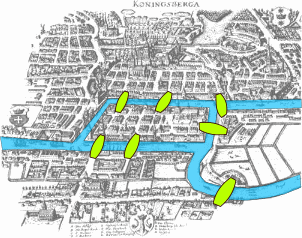
\includegraphics[height=6cm]{Kuva_Sillat_1}
\caption{Könisbergin, nykyisen Kaliningradin, sillat ennen vuotta 1975. \textit{Kuva lähteestä \cite{Sillat_1}} \label{fig:Sillat_1}}
\end{figure}

\begin{figure}[htb]
\centering 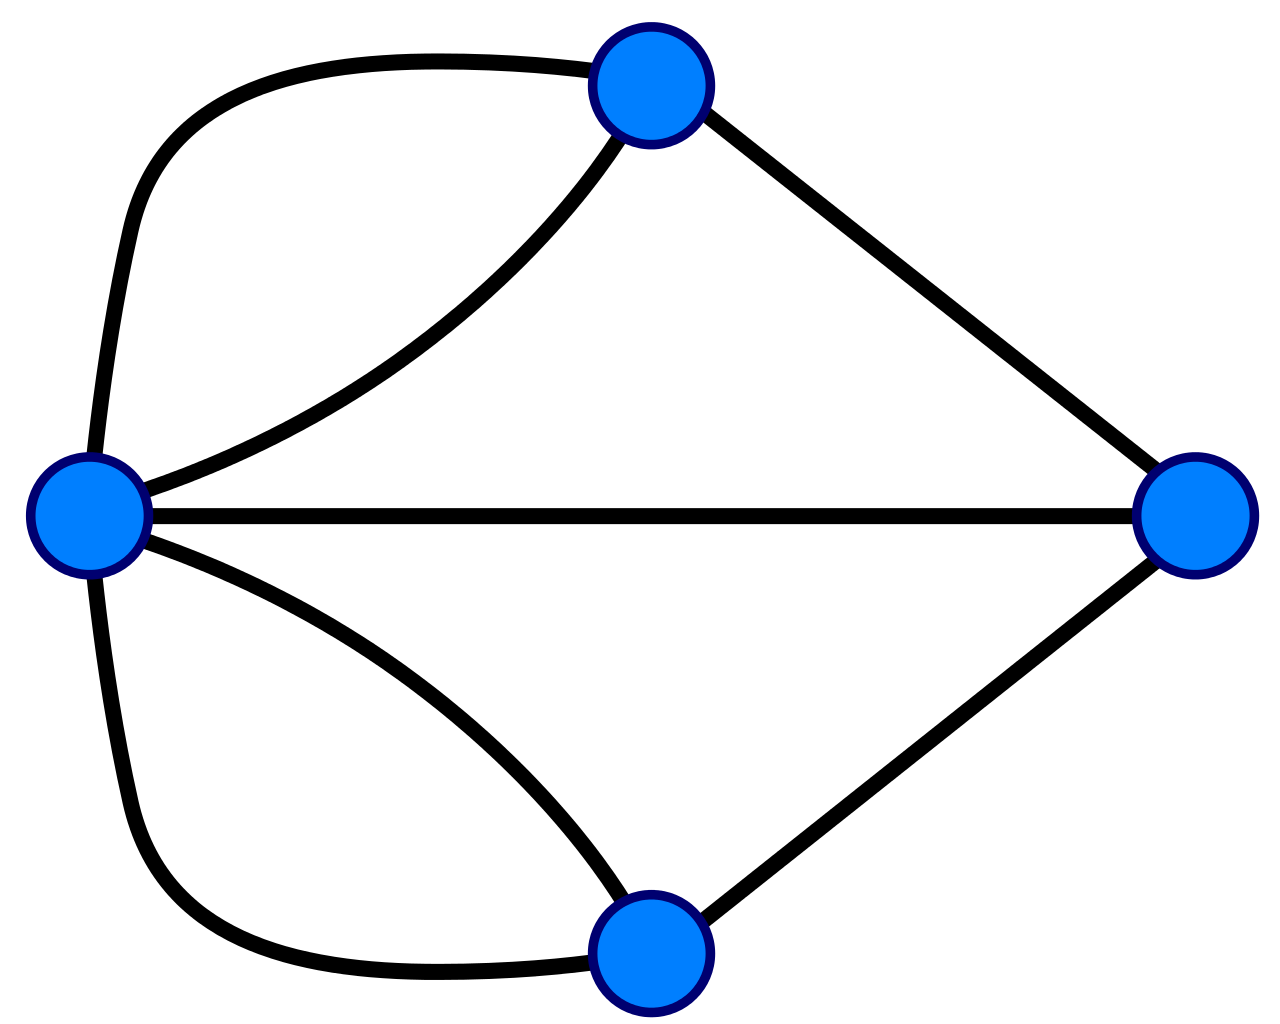
\includegraphics[height=6cm]{Kuva_Sillat_3}
\caption{Könisbergin sillat verkkona. Eulerin todistus ongelmaan: voiko kaikkien seitsemän sillan yli kulkea vain kerran perustuu yksinkertaiseen havaintoon, että solmu jossa on pariton määrä linkkejä voi olla vain reitin alku tai loppupiste ja että reitillä voi olla vain yksi alku- ja loppupiste. Kuitenkin Königsbergin ongelmassa neljällä solmulla on pariton määrä linkkejä, joten ongelmassa kysyttyä reittiä ei ole olemassa \cite[17]{Linkit}. \textit{Kuva lähteestä \cite{Sillat_3}} \label{fig:Sillat_3}}
\end{figure}

Duncan Watts ja Steven Strogatz julkaisivat 1998 ensimmäisen pieni maailma verkostoja käsittelevän artikkelin Naturessa. He esittivät siinä matemaattisen mallin, jolla luodaan verkosto, joka on samaan aikaan hyvin ryvästynyt ja jossa solmujen välinen etäisyys on hyvin pieni verrattuna verkoston kokoon \cite{Collective-dynamics}. Tätä mallia kutsutaan nimillä Watts–Strogatz malli ja Wattsin $\beta$ -malli. Jälkimmäinen nimi tulee Wattsin populaari tiedekirjasta Six Degrees \cite{Six-Degrees}. Mallissa lähdetään liikkeelle verkosta, jossa solmut ovat asettuneet ympyrän kehälle ja ne ovat linkittyneet vain muutamaan lähimpään naapuriinsa. Tässä vaiheessa mallin verkosto on siis täysin järjestynyt. Tämän jälkeen verkosta valitaan satunnaisesti kaksi solmua ja muodostetaan niiden välille linkki. Kun tätä toistetaan muutaman kerran, muuttuu verkoston topologia dramaattisesti. Esimerkiksi kun alkuperäinen ympyrä sisältää 1000 solmua, jotka kaikki on linkitetty 10 lähimpään solmuun, ja kun tähän verkostoon lisätään 10 linkkiä satunnaisesti, putoaa verkoston solmujen keskimääräinen etäisyys 50:stä noin 7:ään. Samaan aikaa verkoston ryvästyneisyys vähenee vain 0,67:stä 0,65:een. Watts ja Strogatz alkoivat kutsua tällaisia pienen etäisyyden ja suuren ryvästyvyyden verkostoja pieni maailma verkostoiksi. \cite{Collective-dynamics}


\begin{figure}[htb]
\centering 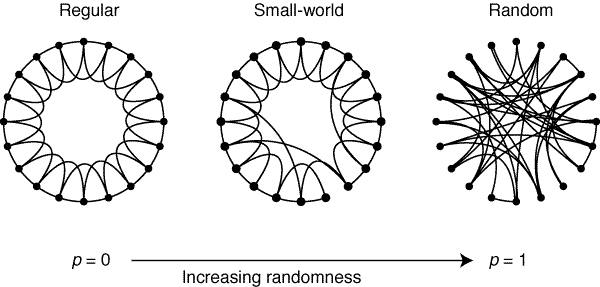
\includegraphics[height=6cm]{Kuva_Collectived_namics_1}
\caption{Vasemmassa laidassa on täysin järjestynyt verkko, keskellä Wattsin $\beta$ -mallin tuottama pieni maailma verkosto ja oikealla satunnainen verkosto. Verkostojen satunnaisuus $p$ kasvaa vasemmalta oikealla. \emph{Lähteestä Watts, Duncan J. ja Strogatz, Steven H. \cite{Collective-dynamics}}\label{fig:Collectived_namics_1}}
\end{figure}


Muillakin verkostoilla voi olla pieni maailma -ominaisuus, joka tarkoittaa, että solmujen välinen keskimääräinen etäisyys on pieni. Esimerkiksi täysin satunnaisella verkostolla on tämä ominaisuus \cite[45]{Nexus}. Pieni maailma verkostot ovat sen lisäksi myös hyvin ryvästyneet ja sen vuoksi niiden solmujen välinen etäisyys on hyvin pieni ja samaan aikaan ne ovat paikallisesti hyvin tiheitä. Näiden ominaisuuksien ansiosta pieni maailma verkostot ovat hyvin ainutlaatuisia. Ne mahdollistavat tiiviin vuorovaikutuksen läheisten solmujen kanssa ja samalla säilyttävät verkoston etäisyydet pieninä.




\begin{figure}[htb]
\centering 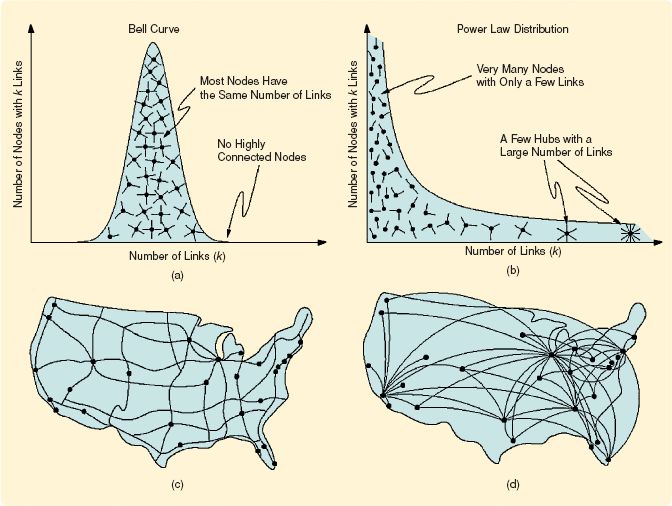
\includegraphics[height=11cm]{Barabasi_1}
\caption{Vertailu satunnaisen ja pieni maailma verkoston rakenteesta ja solmujen linkkien lukumäärästä. (a) Satunnaisen verkoston solmujen lukumäärän (Number of Nodes with Links) jakauma solmun linkkien lukumäärän (Number of Links) suhteen. (b) Pieni maailma verkoston solmujen lukumäärän jakauma solmujen linkkien lukumäärän suhteen. (c) Yhdysvaltain valtatieverkosto on likimain satunnainen verkosto. (d) Yhdysvaltain lentoreittien verkosto on pieni maailma verkosto. Satunnaisen verkoston jakauma (a) noudattaa normaalijakaumaa, eli Gaussin kellokäyrää (Bell Curve), kun taas pieni maailma verkoston jakauma noudattaa eksponenttijakaumaa, josta seuraa, että satunnaisessa verkostossa ei ole solmuja (No Higly Connected Nodes), kun taas pieni maailma verkostossa niitä on vähän (A Few Hubs with a Large Number of Links).  \textit{Lähteestä A. l. Barabasi \cite{The-Architecture}} \label{fig:Barabasi_1}}
\end{figure}

Pieni maailma verkostot ovat mittakaavattomia verkostoja. Mittakaavaton verkosto, josta käytetään myös nimeä skaalautumaton verkosto, ei nimensä mukaisesti skaalaudu, eli sen rakenne ei muuttuu sen koon muuttuessa. Toisin sanoen siltä puuttuu mittakaava, eli sen solmujen linkkien lukumäärät muuttuvat verkoston koon kasvaessa. Näin ollen verkoston rakennetta ei voi päätellä mistään sen osaverkoston rakenteesta. \cite[74--76]{Linkit} Mittakaavattoman verkoston solmujen linkkien lukumäärä noudattaa potenssijakaumaa, jonka merkittävin ero normaalijakaumaan on ääriarvojen esiintyminen useammin. Esimerkiksi lentokentät muodostavat mittakaavattoman verkoston, jossa pääosa liikenteestä keskittyy pääkentille. \cite[74--76]{Linkit}


Mittakaavallinen verkosto, esimerkiksi täysin satunnainen verkosto, puolestaan on rakenteeltaan tasaisempi. Sen rakenne pysyy samana, oli sen koko mikä tahansa. Näin ollen koko verkoston rakenne on sama kuin sen osaverkostojen rakenne. Mittakaavallisen verkoston solmujen linkkien lukumäärä noudattaa normaalijakaumaa, eikä linkkien lukumäärässä esiinny juuri ääriarvoja. Sen sijaan lähes kaikki solmut ovat lähellä keskivertoa.


\begin{figure}[htb]
\centering 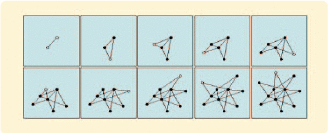
\includegraphics[height=5cm]{Barabasi_2}
\caption{Mittakaavaton verkosto syntyy kuin itsestään, kun verkostoon lisätään solmuja yksitellen. Lisätyt solmut linkittyvät todennäköisimmin näihin solmuihin, jossa on jo paljon linkkejä. \textit{Lähteestä A. l. Barabasi \cite{The-Architecture}} \label{fig:Barabasi_2}}
\end{figure}

Mittakaavattomat verkostot syntyvät usein dynaamisissa, eli ajan myötä kehittyvissä prosesseissa. Kun verkostoon lisätään solmuja yksitellen, ja lisättävät solmut muodostavat linkkejä verkostossa jo oleviin solmuihin, syntyy mittakaavattomia verkostoja, mikäli tämä kytkeytymistodennäköisyys eri solmuihin riippuu niillä jo olevien linkkien lukumäärästä. Tämä prosessi on esitetty kuvassa \ref{fig:Barabasi_2}.  Pieni maailma verkostot voivat olla myös mittakaavattomia verkostoja, jolloin ne syntyvät tällä tavalla. Suurin osa todellisen maailman verkostoista kasvaa ajan myötä, ja tämä on yksi syy miksi pieni maailma verkostoja syntyy mitä erilaisimpiin paikkoihin aina www-sivuista ekosysteemeihin. Merkittävä mittakaavattomien verkostojen ominaisuus on se, että niistä voi löytyä napoja, joilla on merkittävästi enemmän linkkejä kuin muilla verkoston solmuilla. Solmut ovat yleensä verkoston vanhimpia solmuja, tai niiden kelpoisuus, eli kyky hankkia uusia linkkejä on suurempi kuin muilla solmuilla. Usein solmujen kelpoisuus riippuu niillä jo olevien linkkien lukumäärästä. Tämä synnyttää rikkaat rikastuu -ilmiön, jossa paljon linkkejä omaavat solmut saavat niitä tulevaisuudessa vielä enemmän. \cite[117]{Nexus} Pieni maailma verkostoissa ei välttämättä ole napoja, se riippuu niiden syntymekanismeista. Kuitenkin suurin osa eri systeemejä kuvaavista verkostoista sisältää napoja. Tämä rakenne on seurausta verkoston kehittymisestä vaiheittain ja rikkaat rikastuu -ilmiöstä. \cite[118]{Nexus}

Sosiaalisissa verkostoissa linkeillä voidaan ajatella olevan painoarvo, joka kuvaa sosiaalisen suhteen voimakkuutta. Hyvän päivän tuttavuuksilla on pieni paino ja kaverisuhteilla suuri ja niin edelleen. Kaverisuhteet muodostavat verkoston rypäät, ja heikot linkit yhdistyvät napoihin ja muihin kaukaisempiin tuttavuuksiin. Heikot linkit ovat myös ne, jotka luovat verkostoon pieni maailma ominaisuuden. Jos heikot linkit poistetaan, verkosto hajoaisi pieniin itsenäisiin rypäisiin. \cite[55]{Nexus} Heikkojen linkkien merkitystä on myös tutkittu esimerkiksi ihmisten työn saannissa ja on havaittu, että lähes kaikki työpaikat kuullaan satunnaisilta tuttavuuksilta eikä niinkään kavereilta \cite{Linkit}. Tämä on luonnollista, sillä tiiviit kaveri- ja perheporukat jakavat usein hyvin läheisen elämän kokemuksen, mutta satunnaisilta tuttavuuksilta kuulee laajemmin muun muassa työelämän mahdollisuuksista. \cite{Linkit}

Pieni maailma verkostoja voidaan käyttää monien erilaisten ilmiöiden mallintamiseen. Esimerkiksi luonnolliset kielet ovat järjestäytyneet pieni maailma verkostoksi. Englanninkielen noin 500 000 käytetyimmän sanan nähdään muodostavan tällaisen verkoston. Sanojen ajatellaan olevan linkittyneen toisiinsa silloin, kun ne esiintyvät tekstiaineistossa peräkkäin. Pieni määrä sanoja kuten "at"\space ja "the"\space muodostavat verkoston navat, ja keskimääräinen etäisyys sanoilla on noin 3. Samankokoisessa satunnaisessa verkostossa tämä tunnusluku olisi myös sama, mutta verkoston ryvästyvyys olisi tuhansia kertoja pienempi. \cite[88]{Nexus} Pieni maailma verkostoja on myös löydetty aivoalueiden välisten kytkentöjen verkostoista, \cite[65]{Nexus} yritysten johtajien suhteista \cite[119]{Nexus}. On myös esitetty, että monien sairauksien kuten syövän \cite{p53-network} hoito vaatii niiden ymmärtämistä systeemisenä ongelmana, joka vaatii niiden tarkastelun pieni maailma verkostona.



\clearpage
\section{Tutkimusaineisto ja -menetelmät}

Sosiaalisten verkostojen tutkimuksen voidaan katsoa jakautuneen kahteen hyvinkin erilaiseen osaan. Toisaalla on avoin lähinnä eri yliopistoissa tehty tutkimus, jossa tieteellisen tavan mukaisesti sekä aineisto, menetelmät, että tulokset ovat julkisesti saatavilla ja arvioitavissa. Toisaalla taas on eri yritysten data-analyytikkojen ja -tieteilijöiden tekemät tutkimukset. Näissä tutkimuksissa tulokset ovat usein ainoa julkisesti saatavilla oleva materiaali, joskin se saattaa erota yrityksen markkinointimateriaalista vain hieman. Toisinaan näiden tutkimusten menetelmät on selvitetty riittävällä tarkkuudella, mutta lähes koskaan tutkimuksen aineistoa ei ole saatavilla, sillä yritykset kokevat aineiston ja sen sisältämän tiedon olevan hyvin tärkeää omaisuuttaan. Kuitenkin suurten kansainvälisten yritysten hallussa olevan aineiston koko antaa mahdollisuuden tutkia sosiaalisia verkostoja täysin uudella tasolla. Tämän vuoksi olen ottanut työhöni käsiteltäväksi Facebookin tutkimuksen \ref{subsec:Kuusi erottavaa askelta}, jossa tutkittiin 1,59 miljardin ihmisen kaverisuhteita. Tyypillisen julkisen tutkimuksen aineisto on usein vain joitakin miljoonia ihmisiä.

\clearpage
\section{Tulokset}


\subsection{Pieni maailma verkostot yritysten rakenteena}

Tunnetun taloustieteilijän Adam Smithin mukaan työn tuottavuus kasvaa erikoistumisen seurauksena, eli sen vuoksi, että jokainen työntekijä oppii tekemää oman osa-alueensa työstä yhä paremmin ja paremmin, eikä hänen täydy käyttää aikaansa muiden työn osa-alueiden opetteluun. Hänen mukaansa talous kasvaa, kun vapailla markkinoilla voidaan vaihtaa työtä ja työn tuotteita ja näin päästä käsiksi muiden erikoistumiseen. Hänen mukaansa vapaat markkinat ovat myös tehokkain tapa kohdistaa yhteiskunnan resursseja. \cite{Kansojen-Varallisuus}

Avoimeksi kysymykseksi hän jätti sen, miksi hierarkkiset yritykset pärjäävät avoimilla markkinoilla. Toisin sanoen miksi hierarkkinen yritys, joka tekee myös sen parhaan osaamisalueensa ulkopuolisia toimintoja, kuten työllistää esimiehiä, pärjää markkinoilla toimijoille, jotka ostavat kaiken markkinoilta, jolloin niiden siis pitäisi Smithin mukaan saada hankittua kaiken toimintansa hierarkkisia yrityksiä paremmin. Lisäksi miksi työn eri osa-alueisiin erikoistuneiden työläisten on kannattavaa toimia yrityksen hierarkian alaisuudessa, eikä myydä työpanostaan avoimilla markkinoilla?

Vastaus tähän löytyy transaktiokustannuksista. Markkinoilta hankittujen resurssien eteen joudutaan tekemään työtä eri tuotteita vertailtaessa ja ostettaessa. Välillä voi siis olla edullisempaa tehdä työ itse kuin hankkia se markkinoilta, sillä sopivan kumppanin löytäminen markkinoilta veisi liikaa resursseja.


\begin{figure}[htb]
\centering 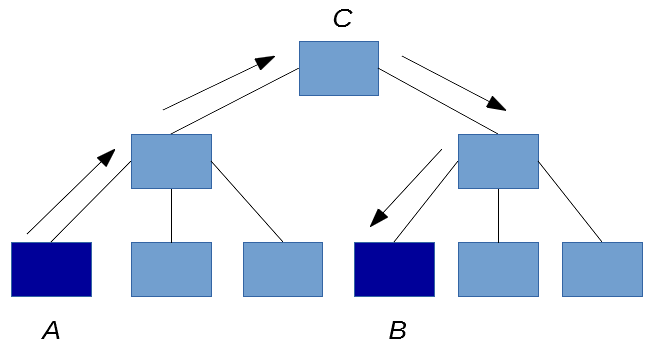
\includegraphics[height=5cm]{Hierarkia_1}
\caption{Viestin kulku hierarkkisessa järjestelmässä. $A$:lta lähetetty viesti joutuu kulkemaan hierarkkisessa järjestelmässä ylempien tasojen kautta. Tämä kuormittaa ylemmillä tasoilla olevia solmuja, ellei viestejä suodateta. Esimerkiksi solmun $C$ kautta kulkisi kaikki hierarkian puolelta toiselle kulkevat viestit. \textit{Kuvan tekijä: Ossi Galkin} \label{fig:Hierarkia_1}}
\end{figure}

Tästä herää kysymys, mikä sitten olisi paras hierarkkinen järjestelmä yrityksille? Puhtaasti hierarkkisessa järjestelmässä hierarkian ylätasoilla olevat yksilöt kuormittuvat helposti hierarkiassa kulkevista viesteistä. Tätä on kuvattu kuvassa \ref{fig:Hierarkia_1}, missä henkilö $A$ lähettää viestin, joka päätyy henkilölle $B$. Kaikki hierarkiassa vaakasuunnassa kulkevat viestit kulkisivat huipun $C$ lävitse, ellei viestejä suodatettaisi. Ja vaikka suodattamisessa onnistuttaisiin, hierarkian eri tasoilla toimivat henkilöt saattavat oppia tehtävänsä liiankin hyvin, mikä johtaa hierarkian jäykkyyteen, sillä ihmiset oppivat tekemään vain oman osa-alueensa hommia. Esimerkiksi varhaisissa Fordin autotehtaissa, jotka olivat maailman ensimmäisiä hierarkkisen järjestelmän toteuttaneita tehtaita, pienikin muutos tehtävissä autoissa saattoi pysäyttää tehtaan viikoiksi. \cite[194]{Linkit}

Hierarkkiset järjestelmät soveltuvat teolliseen massatuotantoon, jossa tiedetiin ennakolta, mitä pitää tuottaa. Yritykset kehittivät pitkälle optimoituja hierarkkisia järjestelmiä, sillä ne olivat paras tapa järjestää tuotanto. Sen sijaan nykyisin suurempi ongelma yrityksille on se, mitä tulisi valmistaa, eikä kuinka halvalla se voidaan valmistaa, sillä suurin osa asioista voidaan jo nykyään tuottaa kyllin halvalla. Tämä vaatii yrityksien siirtymistä hierarkkisista järjestelmistä verkostomaisiin järjestelmiin, joiden rakenne sallii suuremman ja nopeamman muovautuvuuden. \cite[195]{Linkit}

Voidaan osoittaa, että pieni maailma verkostot ovat tehokkain tapa järjestää viestien kulku organisaatioissa, \cite{Six-Degrees} sillä ne minimoivat viestien välityksestä aiheutuvan kuormituksen. Käytännössä yritykseen tarvitaan rypäinä yhdessä toimivia ihmisiä, sekä pieni määrä nämä rypäät toisiinsa yhdistäviä solmuja, joiden tärkein tehtävä on välittää tietoa yrityksessä. Näitä solmuja kutsutaan yritysmaailmassa yleensä managereiksi. Pieni maailma verkostot soveltuvat organisaatiorakenteeksi muita verkostoja paremmin, sillä niissä solmujen keskimääräinen etäisyys on pieni, jonka ansiosta ne minimoivat viestien välityksestä aiheutuvan kuormituksen.

\subsection{Kuusi erottavaa askelta}
\label{subsec:Kuusi erottavaa askelta}

Vuonna 1967 psykologi Stanley Milgram toteutti kokeen, jossa satunnaisia ihmisiä pyydettiin toimittamaan kirje tietylle henkilölle omaa tuttavuusverkostoaan käyttäen. He siis saivat lähettää kirjeen vain joillekin tuntemalleen henkilölle, joka sai lähettää sen vain omille tutuilleen. Kirjettä ei saanut kuitenkaan lähettää suoraan kohteelle. Milgram ja Travers toistivat kokeen vuonna 1969, ja sen tulos oli sama: kirjeen toimitus vaati keskimäärin viidestä kuuteen lähetystä, jotta se saavutti määränpäänsä. Vaikka tutkimuksia kritisoitiin muun muassa kadonneiden kirjeiden suuren määrän vuoksi, katsottiin niiden todistavan, että sosiaalisista verkostoista löytyy reittejä mielivaltaisten ihmisten välillä ja että nämä reitit ovat suhteellisen lyhyitä. \cite[31]{Linkit}

Ajatus siitä, että maailman ihmiset ovat yhdistetty toisiinsa vain kuudella askeleella, lähti kuitenkin leviämään vasta vuonna 1990, kun kuuluisa yhdysvaltalainen kirjailija kirjoitti siitä näytelmässään, jonka jälkeen ajatusta on toistettu lukemattomissa lähteissä:

\begin{quote}
“I read somewhere that everybody on this planet is separated by only six other people. Six degrees of separation. Between us and everybody else on this planet. The president of the United States. A gondolier in Venice. fill in the names. ... Six degrees of separation between me and everyone else on this planet. But to find the right six people.” \textit{John Guare \cite{Guare_runo}}
\end{quote}

Sosiaalinen media on mahdollistanut ihmisten välisten suhteiden tutkimisen aiempaa helpommin, sillä sosiaalisen median käyttämisestä syntyy tarvittava data ihmisten suhteiden tutkimiseen. Facebookissa käyttäjien pitää hyväksyä toisensa "kavereiksi"\space ennen kuin he voivat aloittaa vuorovaikuttamisen keskenään Facebookissa. Näitä kaveruuksia tutkimalla voidaan päätellä, miten käyttäjien tuttavuusverkostot ovat rakentuneet Facebookissa. Sergey Edunov et al. tutkivat \cite{Three-and-half} käyttäjien keskimääräistä etäisyyttä kaikkien Facebookin käyttäjien välillä. Tutkimuksessa ei laskettu jokaisen ihmisen etäisyyttä jokaiseen muuhun, sillä se olisi ollut laskennallisesti liian haastavaa. Lisäksi pitää huomioida, että jo kavereiden kavereista löytyy paljon henkilöitä, jotka ovat myös pelkästään kavereita. Tämän vuoksi tutkimuksessa käytettiin Flajolet-Martin -algoritmia, jossa jokaiselle solmulle annetaan oma tiivistearvo. Puolelle ihmisistä tulee pariton tiiviste, yhdelle neljäsosalle neljällä jaollinen ja niin edelleen. Tämän ansiosta voidaan helposti arvioida, kuinka monta ihmistä saavutetaan kullakin askeleella, sillä parilliset tiivisteet loppuvat binäärimuodossa nollaan, neljällä jaolliset kahteen nollaan ja niin edelleen. Matemaattisesti $(\frac{1}{2})^n$ osalla ihmisistä tiiviste loppuu aina $n$ kappaleeseen nollia. Tämän päättelyn voi kääntää: tarkastelemalla, kuinka monta nollaa enimmillään löytyy tiivisteen lopusta, voidaan päätellä jokaisella askeleella löytyvien ihmisten määrä. Toisin sanoen $n$ määrällä nollia löytyy $c \cdot 2^n$ uniikkia ihmistä. Tämän algoritmin avulla etäisyyden laskeminen onnistuu vain etsimällä kullakin askeleella löytyvien tiivisteiden arvoista se, jonka perässä on eniten nollia. Tätä toistetaan rekursiivisesti ensin kavereille, sitten kavereiden kavereille ja niin edelleen. Näin saadaan pääteltyä, kuinka monta ihmistä kullakin askeleella voidaan tavoittaa.

\begin{figure}[htb]
\centering 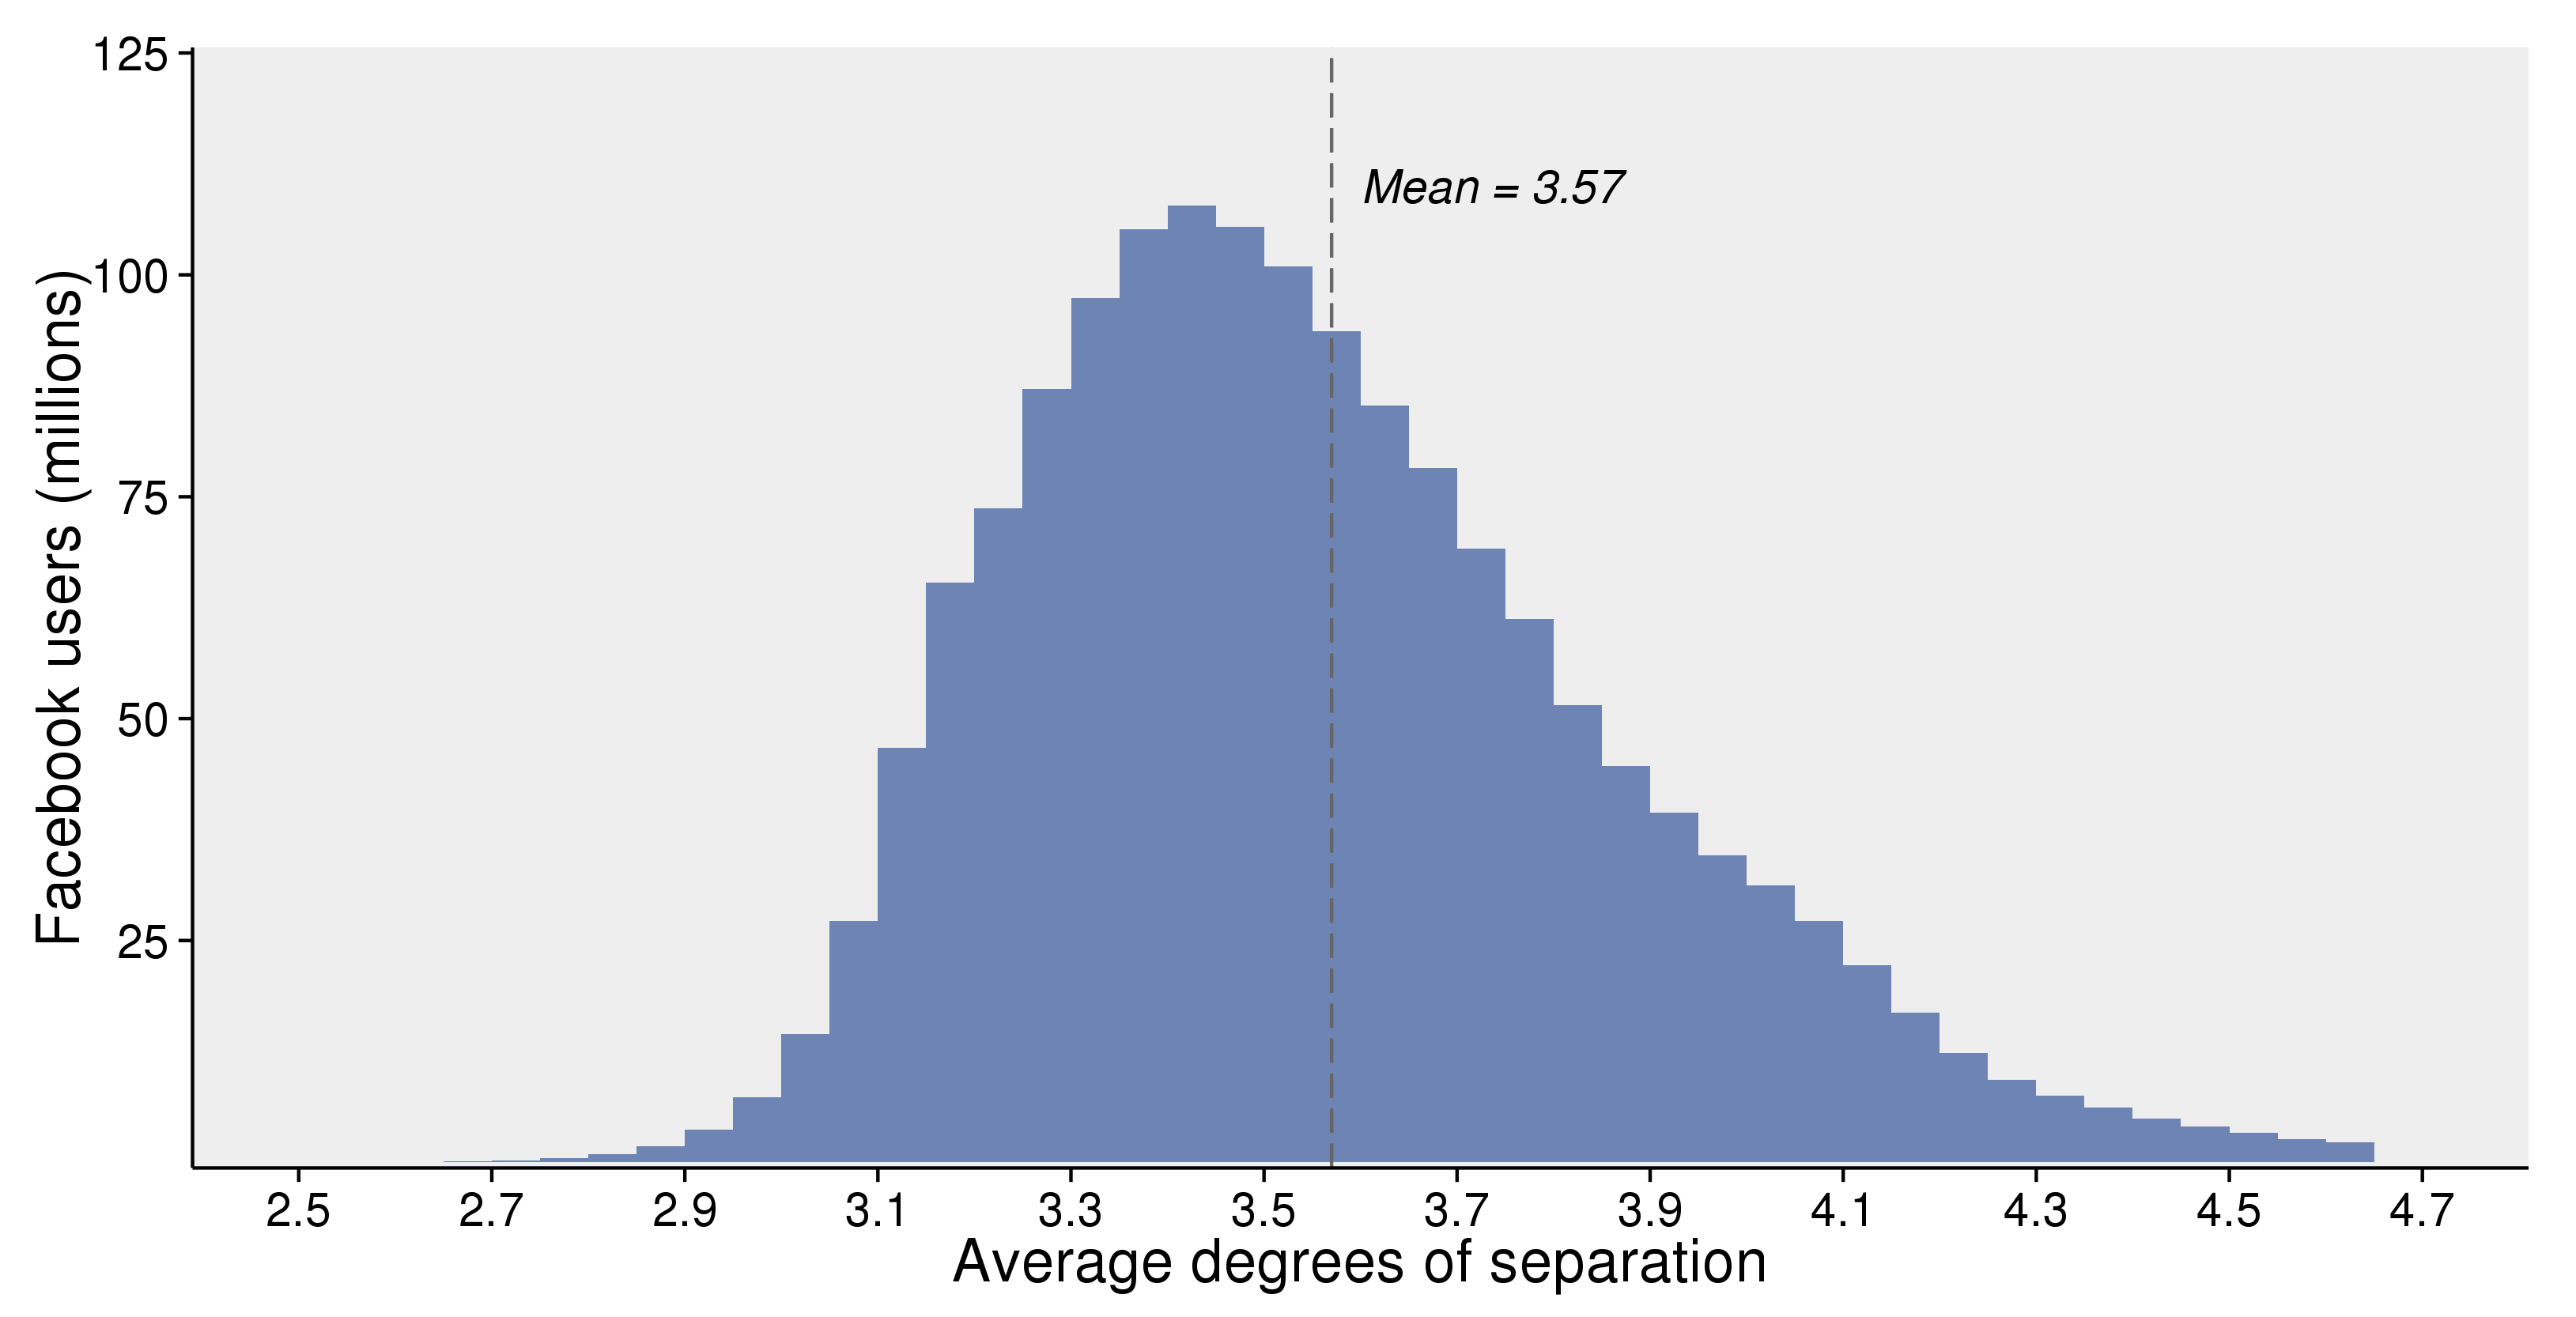
\includegraphics[height=8cm]{Kuva_Facebook_1}
\caption{Arvioitu keskimääräinen etäisyys kaikkien Facebookissa olevien ihmisten suhteen. Keskimääräinen henkilö on yhteydessä jokaiseen muuhun keskimäärin 3,57 askeleella. Suurin osa ihmisistä on keskimäärin 3 ja 4 askeleen etäisyydellä. \textit{Lähteestä Edunov et al. \cite{Three-and-half} \label{fig:Facebook_1}}}
\end{figure}

Tutkimuksen mukaan ihmiset olisivatkin keskimäärin erotettu vain $3,57$ askeleella, eikä kuudella niin kuin Milgramin koe osoitti. Ero voi johtua siitä, että Facebookin kaltaisessa sosiaalisessa mediassa kynnys hyväksyä toinen ihminen kaveriksi on alhaisempi kuin kirjeen lähettäminen hänelle, tai siitä, että Facebookissa olevat kaverit eivät unohdu samalla tavalla kuin entiset työ- tai koulukaverit. Tarkemmin tutkimuksen tulokset on esitetty kuvassa \ref{fig:Facebook_1}.

\subsection{Häiriöiden sietokyky}
\label{subsec:Sietokyky}

Pieni maailma verkostoille on voitu johtaa useita analyyttisia tuloksia, jotka paljastavat verkoston ominaisuudet. Nämä ominaisuudet voivat joko parantaa tai heikentää verkoston sietokykyä. Analyyttiset tulokset tarjoavat keinoja estää romahduksen ekologisissa, biologisissa tai taloudellisissa järjestelmissä, ja niitä voidaan käyttää ohjaamaan teknisten järjestelmien suunnittelua. Tällöin järjestelmä saadaan kestämään sisäisiä vikoja ja ympäristömuutoksia.

Yksi tuoreimmista tuloksista on Jianxi Gaon, Baruch Barzelin ja Albert-László Barabásin tutkimus \cite{Universal-resilience}, joka osoitti, että vaikka kompleksiset järjestelmät ovat kuvattavissa moniulotteisten parametriavaruuden omaavalla malleilla, näiden mallien ennusteet koskien verkoston käyttäytymistä erilaisten häiriöiden suhteen, ovat ennalta arvaamattomia ja siten käyttökelvottomia. He kehittivät keinon muuntaa moniulotteiset mallit yksiulotteiseksi malliksi, jossa $\beta_{eff}$ kuvaa verkoston sietokykyä kokonaisuudessaan. He osoittivat, että tämän mallin avulla voidaan paljastaa universaaleja piirteitä verkoston sietokyvyn kuvaamisesta. He johtivat pieni maailma verkostoille yleisesti pätevän yhtälön:

$$\beta_{eff} = \langle s \rangle + \mathcal{S} \mathcal{H}$$

jossa $\langle s \rangle$ on solmujen astelukujen keskiarvo, eli verkoston tiheys, $\mathcal{S}$ on verkoston symmetria ja $\mathcal{H}$ on verkoston heterogeenisyys.

Useimmissa järjestelmissä osasten luontainen käyttäytyminen ja niiden väliset vuorovaikutukset vaikuttavat muuttumattomina häiriöihin. Häiriöt vaikuttavat vain verkoston rakenteeseen, eli siihen minkälaisessa vuorovaikutuksessa solmut ovat toistensa kanssa ja miten voimakkaasti. Malli osoittaa, että verkoston rakenteen merkitys sen sietokyvylle voidaan kokonaisuudessaan esittää $\beta_{eff}$ avulla. He testasivat mallin toimintaa tarkastelemalla erilaisten laskennallisesti tuotettujen verkostojen sietokykyä häiriöille, sekä tarkastelemalla kahden bakteerin geneettisten verkostojen sietokykyä. Nämä tulokset on esitetty kuvassa \ref{fig:Recilience_2}. Malli osoitti, että tiheys, heterogeenisyys ja symmetria ovat kolme keskeistä rakenteellista tekijää, jotka vaikuttavat järjestelmän kestokykyyn. Ne eivät muuta verkoston keikahduspisteitä, mutta työntävät järjestelmää kauas näistä kriittisistä kohdista ja auttavat sitä kestämään suuria häiriöitä. Mallin avulla voi myös kehittää strategioita sietokyvyn säilyttämiseksi ja suunnitteluperiaatteita, joilla verkostoista voidaan suunnitella kestävämpiä. \cite{Universal-resilience}

\begin{figure}[htb]
\centering 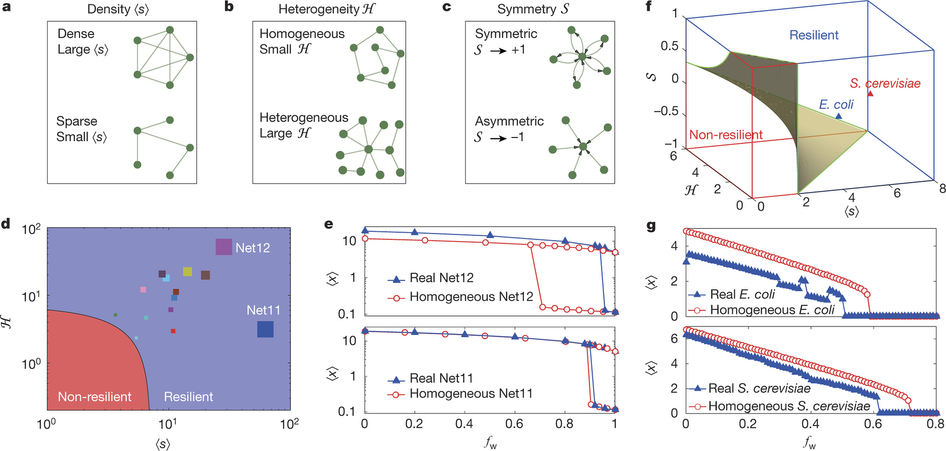
\includegraphics[height=7cm]{Recilience_2}
\caption{Verkoston rakenteen vaikutus sen sietokykyyn. Verkoston rakenteelliset ominaisuudet, jotka vaikuttavat systeemin sietokykyyn $\beta_{eff}$ kautta, ovat \textbf{a} verkoston tiheys $\langle s \rangle$, \textbf{b} verkoston heterogeenisyys solmujen asteina tai linkkien painoina $\mathcal{H}$ ja \textbf{c} symmetria $\mathcal{S}$. \textbf{d} Faasikaavio $\langle s \rangle \mathcal{H}$-tasossa. Suurempi $\beta_{eff}$ (neliö koko) tarkoitti syvemmällä sietokykyisessä tilassa oloa. \textbf{e} Keskimääräinen järjestelmän tila $\langle x \rangle $, keskimääräisen linkkien painojen $fw$ vähenemisen suhteen. Verkko Net12 oli kaikkein heterogeenisin tutkituista ja se vältti sietokykynsä romahtamisen jopa kun $f_w = 97 \%$. Homogeeninen verkko, jossa oli sama tiheys ja $\mathcal{H} = 0$ menetti sietokykynsä kun $f_w = 66\%$ (punaiset ympyrät) täten heterogeenisyys on syy verkon Net12 poikkeukselliselle sietokyvylle. Kuten kuvasta d voidaan päätellä Net11:ta sietokyvyn syy on sen korkeassa tiheydessä $\langle s \rangle $. \textbf{f} Faasidiagrammi säätelyverkostolle, kun siirtyminen elävästä solusta kuolleeseen tapahtuu $\langle s \rangle + \mathcal{S} \mathcal{H} = 2.$ Kuvassa on myös S. cerevisiaen ja E. coli verkostojen sijainti (kolmiot). \textbf{g} molemmille organismeille $\mathcal{S} <0$, ja siten heterogeenisyys vähentää niiden kestokykyä. Homogeeninen verkko (punaiset ympyrät) kestää suurempia häiriöt kuin alkuperäinen verko (siniset kolmiot). \label{fig:Recilience_2} \textit{Lähteestä Gao et al. \cite{Universal-resilience}}}
\end{figure}

 
Aikaisemmin verkostojen tutkimus on paljastanut muun muassa, että sillä, että verkoston navoilla on lähes kaikki heikot linkit on huomattavia vaikutuksia verkoston toimintaan. Esimerkiksi kun on tarkasteltu sukupuolitautien leviämistä, on huomattu, että navat eivät ainoastaan mahdollista tautien leviämistä pitkiä matkoja verkostossa vaan ne muuttavat tautien leviämistä huomattavasti. Alessandro Vespignani ja Romualdo Pastor-Satorras osoittivat, \cite{Epidemic-Spreading} että pieni maailma verkostoissa taudit voivat aina saavuttaa keikahduspisteen, eli aina on mahdollisuus, että taudit alkavat levitä hallitsemattomasti. Taudin leviämisen todennäköisyyteen vaikuttaa monta tekijää: niiden kyky levitä yksilöstä toiseen; niiden tappavuus, jos tauti tappaa isäntänsä liian aikaisin, se ei ehdi leviämään; niiden elinikä, eli montako uutta sukupolvea tauti kykenee tuottamaan elinikänsä aikana; sekä tautia vastaan suunnatut hoidot kuten rokotukset. Tauti, jonka leviämistodennäköisyys on keikahduspisteen alapuolella, katoaa vääjäämättä. Näin siis tapahtuu satunnaisissa verkostoissa. Sen sijaan pieni maailma verkostoissa taudit, oli niiden todennäköisyys levitä kuinka pieni tahansa, voivat levitä koko verkostoon, kunhan ne vain tartuttavat jonkin verkoston navoista. Tämän jälkeen pelkkä napojen linkkien lukumäärä mahdollistaa taudin leviämisen, oli tartuntatodennäköisyys yhtä linkkiä pitkin miten alhainen tahansa. Tästä seuraa, että taudeilta, jotka leviävät mittakaavattomassa pieni maailma verkostoissa, kuten HI-virukselta, ei voida suojautua tarjoamalla lääkkeitä ja rokotteita kaikille sairastuneille ja riskiryhmiin kuuluville \cite{Immunization-of-complex-networks}. Sen sijaan tauteja vastaan voidaan taistella muuttamalla verkoston rakenteita. Tämä voidaan tehdä tekemällä verkoston napoina toimivista ihmisistä immuuneja lääkkeiden ja valistuksen avulla. Kun he eivät enää levitä tautia, loppu osa verkostosta enää ole pieni maailma verkosto ja sillä on oma keikahduspisteensä, jolloin tautien leviämistä voidaan estää perinteisillä hoito- ja rokotusohjelmilla. \cite{Immunization-of-complex-networks} Sukupuolitautien tapauksessa prostituoitujen ja sotilaiden on havaittu välittävän suurimman osan taudeista, joten nämä ihmisryhmät toimivat muun muassa HI-viruksen leviämisen mahdollistajana ja seksuaalisten kontaktien verkoston napoina, jotka hoitamalla viruksen leviäminen voidaan taltuttaa.



\clearpage

\section{Yhteenveto}
%\section{Summary}

Tässä työssä käytiin läpi, miten Duncan Wattsin ja Steven Strogatzin löytämät pitkän matkan linkit muuntavat täysin säännöllisen verkoston pieni maailma verkostoksi. Sekä miten Alber Barabási keksimä yksinkertainen verkoston kasvu, jossa rikkaimmat ja suosituimmat solmut muuttuvat yhä rikkaammiksi ja suosituimmiksi, tuottaa pieni maailma verkostoja, jotka ovat hieman erilaisia kuin edelliset, sillä ne sisältävät napoja. Keskeinen piirre näissä on se, että systeemiin ilmaantuu järjestystä sen osasten vuorovaikutuksesta. Tämä ilmenee esimerkiksi solmujen linkkien määrän potenssijakaumana, eli siinä, että pieni osa solmuista, eli navat, hallitsee suurinta osaa linkeistä. Hyvin monet todellisen maailman systeemit kasvavat ajan kuluessa, ja jos niissä olevin solmujen todennäköisyys saada uusia linkkejä riippuu solmuilla jo olevien linkkien lukumäärästä, syntyy näistä verkostoista pieni maailma verkostoja. Tämän yksinkertaisen syntymekanismin ansiosta pieni maailma verkostoja löytyy mitä erilaisimmista todellisen maailman systeemeistä. Pieni maailma verkostojen keskeinen ominaisuus on suuri ryvästyneisyys eli paikallisesti vuorovaikuttavien solmujen joukot, sekä pieni keskimääräinen etäisyys solmujen välillä. 

Tässä työssä käytiin tarkemmin läpi, miten pieni maailma verkostoja käytetään ihmisen sosiaalisen ympäristön tutkimuksessa. Kuinka tätä tietoa voidaan käyttää hyväksi yrityksien toimintaa suunniteltaessa ja eri verkostojen sietokyvyn parantamisessa, muun muassa suojautumisessa HI-virusta vastaan. Lisäksi tarkasteltiin miten ihmisen sosiaalisen verkoston rakennetta voidaan kartoittaa sosiaalisen median avulla.


% TODOs
% TIIVISTELMÄ ENGLANNIKSI
% jos ja pilkut

\clearpage
%% Lähdeluettelo

% ############################################################################

\addcontentsline{toc}{section}{Viitteet}
%\bibliography{viitteet}
%\bibliographystyle{plain}
\printbibliography
%\pagestyle{plain}


%% Liitteet jos tavitsee
% \clearpage
% \thesisappendix
% \section{Esimerkki liitteestä\label{LiiteA}}
% Liite jos tarvitsee

\end{document}


